In questa sezione verrà discussa una possibile implementazione di una soluzione hardware basata su un approccio non ottimizzato (medesimo a quello iniziale) in cui è stato considerato il protocollo AXI4-Stream. Pertanto, tale solution non è da considerare come ottimizzazione rispetto alle precedenti ma come caso d'uso dello standard in corrispondenza di una delle solution precedentemente citate. In particolare, come già citato per semplicità si farà riferimento alla \textit{Unoptimized Solution}.
\\
Il protocollo AXI4-Stream è utilizzato come interfaccia standard per collegare componenti che desiderano scambiare dati. L'interfaccia può essere utilizzata per collegare un singolo master, che genera dati, a un singolo slave, che riceve dati. Il protocollo può essere utilizzato anche per collegare un numero maggiore di componenti master e slave. Lo standard supporta flussi di dati multipli che utilizzano lo stesso insieme di bus condivisi, consentendo di costruire un'interconnessione generica. In particolare, con l'interfaccia Stream si garantisce un nuovo dato in input ad ogni colpo di clock. In questo caso specifico, quindi, ci si aspetta che lo standard garantisca 11 dati in input per 11 colpi di clock così da essere processati ed essere messi in uscita.

\begin{figure}[H]
	\centering
	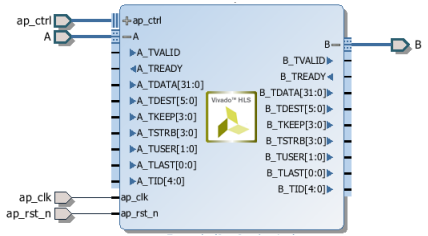
\includegraphics[width=0.7\textwidth]{solutions/axi/axistream.png}
	\caption{AXI4-Stream Protocol}
\end{figure}

Nello specifico, il tipo di pacchetto includerà il segnale corrispondente al dato effettivo e tutti gli altri segnali che servono per lo standard corrispondente.

\lstinputlisting[language=C++]{solutions/axi/fir_axi.cpp}

In particolare, \textit{inputStreamFilter} e \textit{outputStreamFilter} sono rispettivamente lo stream di ingresso e lo stream di uscita all'architettura. 
\\
Per quanto riguarda, invece, le direttive specificate inizialmente, la prima fa riferimento al fatto che il tool non deve sintetizzare i segnali \textit{ap\_ctrl} tranne quella relativa a \textit{inputStreamFilter} e \textit{outputStreamFilter} e i segnali relativi allo standard, mentre la seconda e la terza rispettivamente fanno riferimento al fatto che \textit{inputStreamFilter} e \textit{outputStreamFilter} devono essere mappati secondo lo standard Stream.
\\
Inoltre, si può notare come, all'interno del ciclo while, sia stato specificato un approccio \textit{non blocking}, cioè in riferimento al fatto che non si sa a priori la quantità di dati entranti nel buffer.
\\
Ovviamente, bisogna specificare che il segnale di \textit{TVALID} sarà pari a 1 soltanto nel momento in cui si ha il risultato finale, cioè in corrispondenza dell'accumulo finale.
\\
Effettuando la sintesi, la C/RTL Cosimulation e l'Export RTL si ottengono i seguenti report.

\begin{table}[H]
	\centering
	\begin{minipage}[t]{0.45\linewidth}
		\centering
		\begin{tabular}{|c|c|c|c|}
			\hline
			\textbf{Clock} & \textbf{Target} & \textbf{Estimated} & \textbf{Uncertainty} \\
			\hline
			ap\_clk & 10.00 & 8.742 & 1.25 \\
			\hline
		\end{tabular}
		\caption{HLS AXI Solution Timing Summary (ns)}
		\label{tab:hls-axi-solution-timing-summary}
	\end{minipage}
	\hfill
	\begin{minipage}[t]{0.45\linewidth}
		\centering
		\begin{tabular}{|c|c|c|c|}
			\hline
			\multicolumn{2}{|c|}{\textbf{Latency}} & \multicolumn{2}{|c|}{\textbf{Interval}} \\
			min & max & min & max \\
			\hline
			? & ? & ? & ? \\
			\hline
		\end{tabular}
		\caption{HLS AXI Solution Latency Summary (clock cycles)}
		\label{tab:hls-axi-solution-latency-summary}
	\end{minipage}
\end{table}

Si può notare come la latenza totale e quella relativa al ciclo for presentano un valore pari a \textit{?}, cioè un valore di latenza non noto, dovuto al fatto che l'architettura presenta un approccio \textit{non blocking}. Inoltre, dal momento che è stata prevista una direttiva di pipeline, si può notare come sia stato raggiunto un Initiation Interval pari a 1.

\begin{table}[H]
	\centering
	\begin{tabular}{|c|c|c|c|c|c|c|c|c|}
		\hline
		\multicolumn{1}{|c|}{Loop} & \multicolumn{2}{|c|}{\textbf{Latency}} & \multicolumn{2}{c|}{\textbf{Iteration Latency}} & \multicolumn{2}{c|}{\textbf{Initiation Interval}} & \multicolumn{1}{c|}{\textbf{Trip Count}}  \\
		Name & min & max & min & max & achieved & target &  \\
		\hline
		- loop & ? & ? & 4 & 4 & 1 & 1 & ? \\
		\hline
	\end{tabular}
	\caption{HLS AXI Solution Latency Loops Summary }
	\label{tab:hls-axi-solution-loop-summary}
\end{table}

\begin{table}[H]
	\centering
	\begin{tabular}{|l|c|c|c|c|}
		\hline
		\textbf{Name}    & \textbf{BRAM\_18K} & \textbf{DSP48E} & \textbf{FF} & \textbf{LUT} \\ \hline
		DSP              & -                   & -               & -           & -            \\ 
		Expression       & -                   & 14               & 0           & 380          \\ 
		FIFO             & -                   & -               & -           & -            \\ 
		Instance         & -                   & -               & -           & -            \\ 
		Memory           & 0                   & -               & -          & -            \\ 
		Multiplexer      & -                   & -               & -           & 171          \\ 
		Register         & -                   & -               & 767         & 32            \\ \hline
		\textbf{Total}   & 0                   & 14               & 767         & 583          \\ \hline
		\textbf{Available} & 280               & 220             & 106400      & 53200        \\ \hline
		\textbf{Utilization (\%)} & 0            & 6              & $\sim$0     & 1      \\ \hline
	\end{tabular}
	\caption{HLS AXI Solution Utilization Estimates Summary}
	\label{tab:hls-axi-solution-utilization-estimates-summary}
\end{table}

\begin{table}[H]
	\centering
	\begin{tabular}{|c|c|c|c|c|c|c|c|}
		\hline
		\multicolumn{1}{|c|}{RTL} & \multicolumn{1}{|c|}{Status} & \multicolumn{3}{c|}{\textbf{Latency}} & \multicolumn{3}{c|}{\textbf{Interval}} \\
		&  & min & avg & max & min & avg & max \\
		\hline
		VHDL & Pass & 13 & 13 & 13 & NA & NA & NA \\
		\hline
	\end{tabular}
	\caption{HLS AXI Solution C/RTL Cosimulation Summary }
	\label{tab:hls-axi-solution-cosimulation-summary}
\end{table}

\begin{table}[H]
	\centering
	\begin{minipage}[t]{0.45\linewidth}
		\centering
		\begin{tabular}{|l|r|}
			\hline
			\textbf{Resource} & \textbf{VHDL} \\
			\hline
			SLICE & 231 \\
			\hline
			LUT & 739 \\
			\hline
			FF & 699 \\
			\hline
			DSP & 0 \\
			\hline
			BRAM & 0 \\
			\hline
			SRL & 0 \\
			\hline
		\end{tabular}
		\caption{HLS AXI Solution Export RTL Resource Usage}
		\label{tab:hls-axi-solution-export-rtl-resoruce-usage}
	\end{minipage}
	\hfill
	\begin{minipage}[t]{0.45\linewidth}
		\centering
		\begin{tabular}{|l|r|}
			\hline
			\textbf{Timing} & \textbf{VHDL} \\
			\hline
			CP required & 10.000 \\
			\hline
			CP achieved post-synthesis & 7.269 \\
			\hline
			CP achieved post-implementation & 8.202 \\
			\hline
		\end{tabular}
		\caption{HLS AXI Solution Export RTL Final Timing}
		\label{tab:hls-axi-solution-export-rtl-final-timing}
	\end{minipage}
\end{table}

Pertanto, importando l'IP in Vivado e impostando un clock constraint pari a 10ns è possibile analizzare i seguenti report di risorse, timing, potenza dinamica ed energia per singola operazione.
\lstinputlisting[language=VHDL]{solutions/axi/clk_constraint.xdc}
In particolare, si può effettuare un confronto rispetto alla soluzione iniziale non ottimizzata, considerata come riferimento per questa implementazione, per valutare gli effetti dell'introduzione del protocollo AXI nell'architettura in questione. Si può notare un aumento dell'utilizzazione delle LUT circa pari al $169\%$ e un aumento del numero di FF circa pari al $337\%$. 
\begin{table}[H]
	\centering
	\begin{tabular}{|c|c|c|c|c|c|c|}
		\hline
		\textbf{LUT} & \textbf{LUTRAM} & \textbf{FF} & \textbf{BRAM} & \textbf{DSP} & \textbf{IO} & \textbf{BUFG} \\
		\hline
		739 & 0 & 699 & 0 & 0 & 93 & 1 \\
		\hline
	\end{tabular}
	\caption{Vivado AXI Solution Utilization Report [\#]}
	\label{tab:vivado-axi-solution-utilization-report}
\end{table}

Si può evidenziare come il numero di cicli previsto per questa soluzione sia pari a 11 come ipotizzato inizialmente.

\begin{table}[H]
	\centering
	\begin{tabular}{|c|c|c|c|}
		\hline
		\textbf{Cycles} [\#] & \textbf{Clock Constraint} [ns] & \textbf{WNS} [ns] & \textbf{Maximum Clock Frequency} [Mhz] \\
		\hline
		11 & 10 & 1.369 & 115.8614297 \\
		\hline
	\end{tabular}
	\caption{Vivado AXI Solution Timing Report}
	\label{tab:vivado-axi-solution-timing-report}
\end{table}

Per quanto riguarda la potenza dinamica totale e l'energia per singola operazione, si può notare un aumento rispetto alla soluzione dove non è presenta la logica di controllo relativa al protocollo AXI. In particolare, notevoli aumenti si hanno in corrispondenza dei contributi di \textit{Clocks}, \textit{Logic} e \textit{Data}.

\begin{table}[H]
	\centering
	\begin{tabular}{|c|c|c|c|c|c|c|}
		\hline
		\textbf{BRAM} & \textbf{Clock Enable} & \textbf{Clocks} & \textbf{DSP} & \textbf{Logic} & \textbf{Set/Reset} [mW] & \textbf{Data} \\
		\hline
		0 & 0.361682673 & 2.409646753 & 0 & 7.963255048 & 0.008282737 & 5.53872576 \\
		\hline
	\end{tabular}
	\caption{Vivado AXI Solution Dynamic Power Report [mW]}
	\label{tab:vivado-axi-solution-dynamic-power-report}
\end{table}

\begin{table}[H]
	\centering
	\begin{minipage}[t]{0.45\linewidth}
		\centering
		\begin{tabular}{|c|}
			\hline
			\textbf{Dynamic Total} \\
			\hline
			16.28159297 \\
			\hline
		\end{tabular}
		\caption{Vivado AXI Solution Dynamic Power Report [mW]}
		\label{tab:vivado-axi-solution-total-dynamic-power-report}
	\end{minipage}
	\hfill
	\centering
	\begin{minipage}[t]{0.45\linewidth}
		\centering
		\begin{tabular}{|c|}
			\hline
			\textbf{Energy Single Operation} \\
			\hline
			162.8159297 \\
			\hline
		\end{tabular}
		\caption{Vivado AXI Solution Energy Single Operation Report [pJ]}
		\label{tab:vivado-axi-solution-energy-single-operation-report}
	\end{minipage}
\end{table}